\documentclass[a4paper,11pt,titlepage]{article}

\usepackage[utf8]{inputenc} 
\usepackage[T1]{fontenc}      
\usepackage[francais]{babel} 
\usepackage[top=4cm, bottom=4cm, left=4cm, right=4cm]{geometry}
\usepackage{graphicx}

\title{Le numérique dans l'accomplissement des SDGs}
\author{Djavan Sergent}

\begin{document}
	\maketitle
	\tableofcontents
	\listoffigures
	\listoftables
	
	\section*{Abstract}
		abstract
	
	\section{Introduction}
		En 2000, les Nations-Unies lancent le programme des Millenim Developpment Goals (MDGs) qui s'étend jusq'en 2015. Il s'agit d'un ensemble d'objectifs internationaux parmi lesquels on peut notamment citer l'éradication de l'extrême pauvreté et de la faim, combattre la mortalité infantile ou encore apporter une éducation à toutes et tous. Les 191 états membres des Nations-Unies ainsi que 22 organisations internationnales se sont engagées à participer activement à la réalisation de ces objectifs.
		\begin{figure}
			\begin{center}
				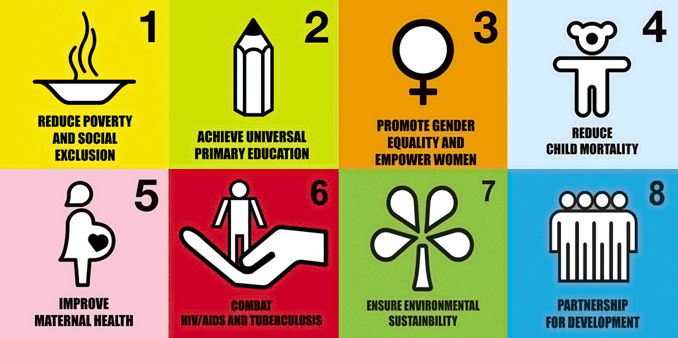
\includegraphics[width=200pt]{mdgs-full.png}
			\end{center}
			\caption{Représentation des MDGs}
		\end{figure}

		La situation en 2015 était que beaucoup d'efforts ont été investis, mais les progrès sont encore très inégaux. Les différents pays membres des Nations-Unies ainsi que des organisations civiles se sont donc intéressées à l'agenda post-2015, c'est à dire aux objectifs futurs. Les Sustainable Developpment Goals (SDGs) ont étés acceptés comme relève des MDGs. Ceux-ci comportent 17 buts, chacuns subdivisé en objectifs. Les SDGs totalisent 169 objectifs possédant chacuns leurs propres indicateurs.
		\begin{figure}
			\begin{center}
				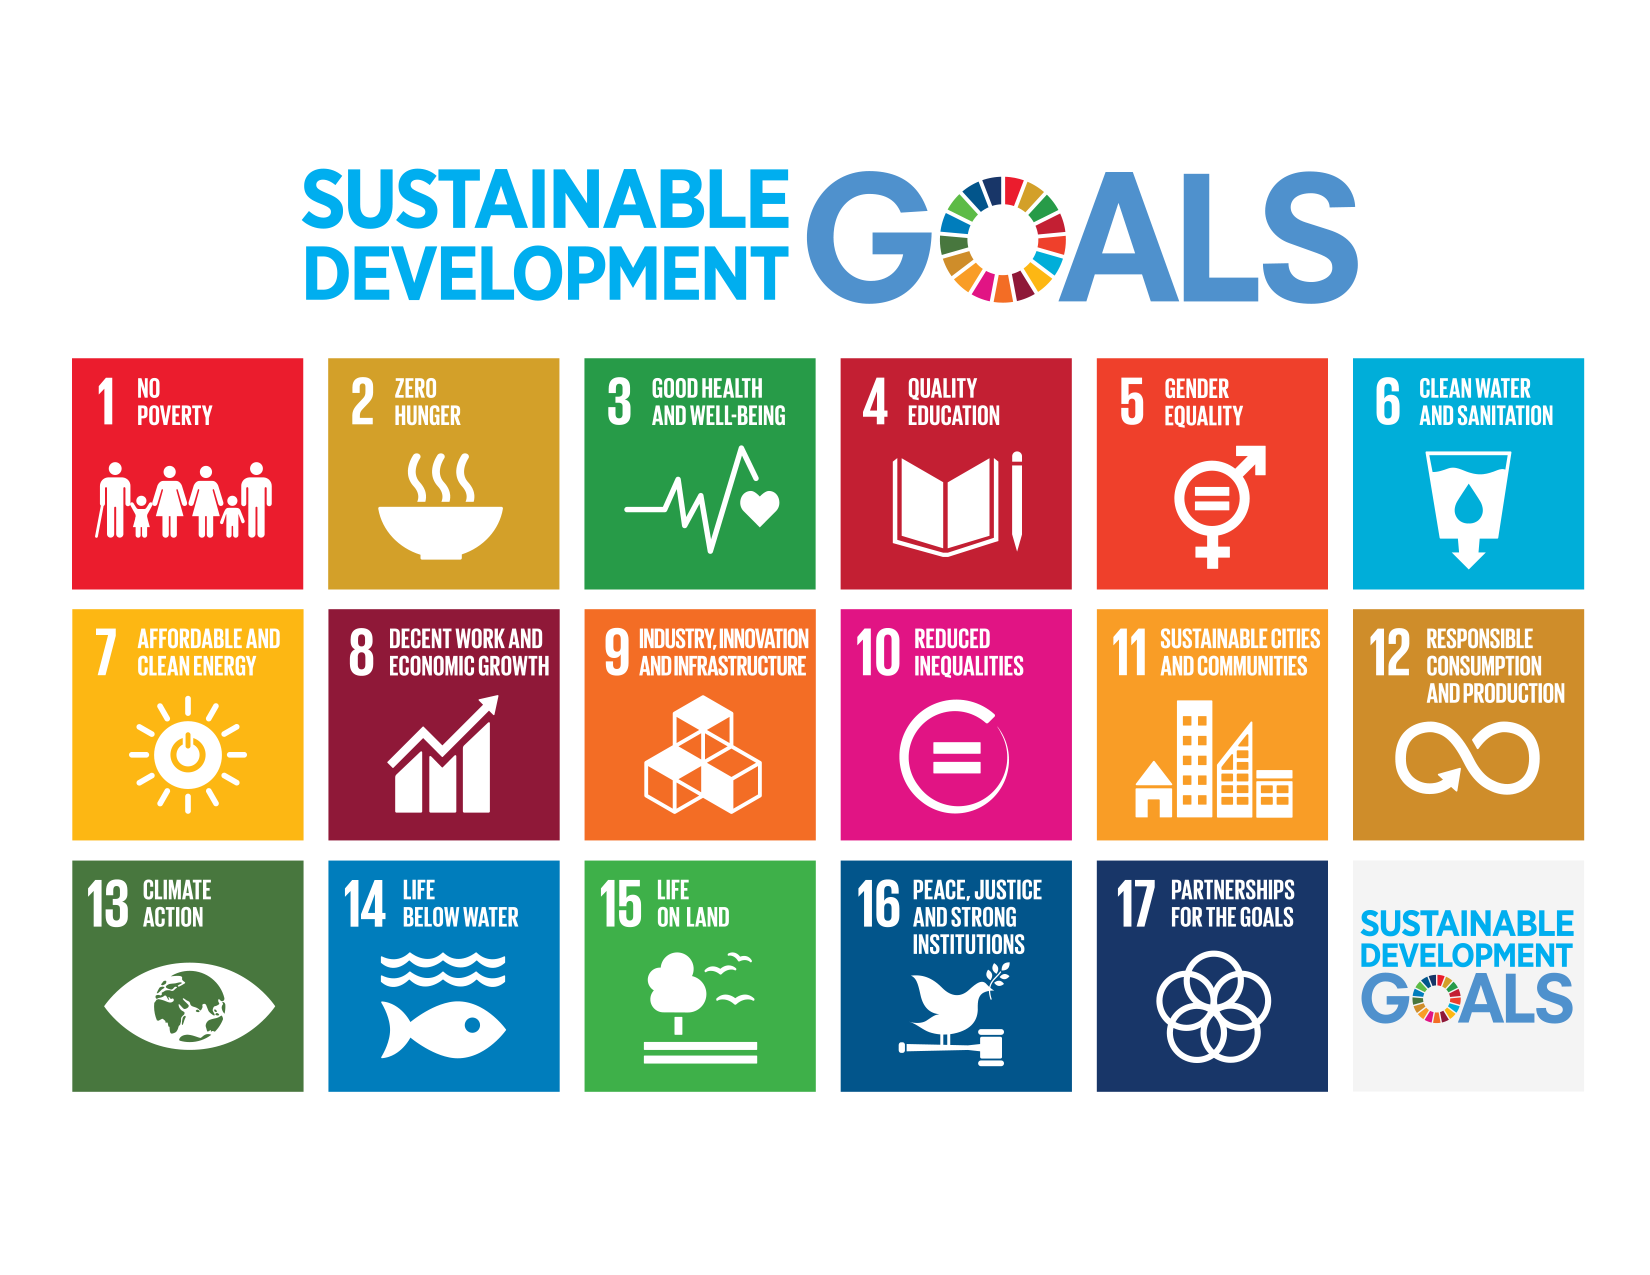
\includegraphics[width=200pt]{sdgs.jpg}
			\end{center}
			\caption{Représentation des SDGs}
		\end{figure}
		
		Nous analysons dans cet article le rôle du numérique dans la réalisation et le monitoring de certains de ces objectifs, particulièrement du point de vue de la participation citoyenne.
		 
		\subsection{Sustainable Developpment Goals}
			\subsubsection{Objectifs}
				Nous nous intéressons, dans le cadre de cet article, aux objectifs suivants :
				\begin{itemize}
					\item 3 : Good-Health and Well-Being
					\item 6 : Clean water and sanitation
					\item 12 : Responsible consumption and production
					\item 13 : Climate Action
					\item 14 : Life below water
					\item 15 : Life on land
				\end{itemize}

			\subsubsection{Indicateurs}
			Pour chaque objectif
			\subsubsection{Progrès et revue}
			\subsubsection{High-Level Political Forum}
			
		\subsection{IT}
	
	\section{Monitoring environnemental et sociétal}
		\subsection{Indicateurs}
			\subsubsection{Métriques}
			\subsubsection{Définitions quantitatives}
			\subsubsection{Impact environnemental}
			\subsubsection{Méthodes}			
			\subsubsection{Limites}
			
		\subsection{Monitoring environnemental}
			\subsubsection{Eau}
				La qualité de l'eau est un élément important à contrôler
			\subsubsection{Air}
			\subsubsection{Territoire}
			\subsubsection{Biodiversité}
		
		\subsection{Monitoring sociétal}
			\subsubsection{Santé}
			\subsubsection{Société}
			
	\section{Participation citoyenne}
		\subsection{Standards}
		\subsection{Récupération de données}
		\subsection{Traitement des données}
		\subsection{Outils}
			\subsubsection{Hardware}
			\subsubsection{Software}
				INatrualist, NatureBytes, Epicollect, SeeClickFix, Water Reporter, Project Noah	
			
	\section{Projets}
		\subsection{Aqueduct}
		\subsection{InfoAmazonia}
		\subsection{World Water Monitoring Day}
		\subsection{Riverfly Monitoring Initiative}
		\subsection{Restoration Assessment Initiative}
		\subsection{Homebrew Sensing Project}
		\subsection{Open Water Project}
		\subsection{Open Air}
		\subsection{Open Land}
	
	\section{Conclusion}
	\newpage
	\bibliographystyle{abbrv}
	\bibliography{biblio}
	

\end{document}